% !TEX encoding = UTF-8
% !TEX TS-program = pdflatex
% !TEX root = ../tesi.tex
% !TEX spellcheck = it-IT

%**************************************************************
\chapter{Analisi dei requisiti}
\label{cap:analisi-requisiti}
%**************************************************************

\intro{Breve introduzione al capitolo}\\

\section{Casi d'uso}

Per lo studio dei casi di utilizzo del prodotto sono stati creati dei diagrammi.
I diagrammi dei casi d'uso (in inglese \emph{Use Case Diagram}) sono diagrammi di tipo \gls{uml} dedicati alla descrizione delle funzioni o servizi offerti da un sistema, così come sono percepiti e utilizzati dagli attori che interagiscono col sistema stesso.
Essendo il progetto finalizzato alla creazione di un tool per l'automazione di un processo, le interazioni da parte dell'utilizzatore devono essere ovviamente ridotte allo stretto necessario. Per questo motivo i diagrammi d'uso risultano semplici e in numero ridotto.

\begin{figure}[!h] 
    \centering 
    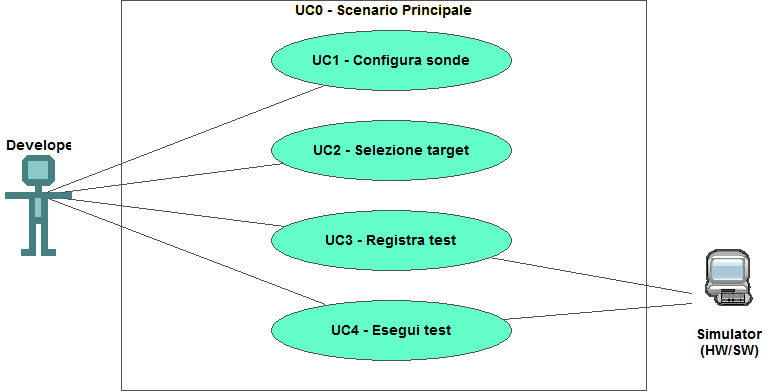
\includegraphics[width=0.9\columnwidth]{usecase/scenario-principale} 
    \caption{Use Case - UC0: Scenario principale}
\end{figure}

\begin{usecase}{0}{Scenario principale}
\usecaseactors{Sviluppatore applicativi}
\usecasepre{Lo sviluppatore è entrato nel plug-in di simulazione all'interno dell'IDE}
\usecasedesc{La finestra di simulazione mette a disposizione i comandi per configurare, registrare o eseguire un test}
\usecasepost{Il sistema è pronto per permettere una nuova interazione}
\label{uc:scenario-principale}
\end{usecase}

\section{Tracciamento dei requisiti}

Da un'attenta analisi dei requisiti e degli use case effettuata sul progetto è stata stilata la tabella che traccia i requisiti in rapporto agli use case.\\
Sono stati individuati diversi tipi di requisiti e si è quindi fatto utilizzo di un codice identificativo per distinguerli.\\
Il codice dei requisiti è così strutturato R(F/Q/V)(N/D/O) dove:
\begin{enumerate}
	\item[R =] requisito
    \item[F =] funzionale
    \item[Q =] qualitativo
    \item[V =] di vincolo
    \item[N =] obbligatorio (necessario)
    \item[D =] desiderabile
    \item[O =] opzionale
\end{enumerate}
Nelle tabelle \ref{tab:requisiti-funzionali}, \ref{tab:requisiti-qualitativi} e \ref{tab:requisiti-vincolo} sono riassunti i requisiti e il loro tracciamento con gli use case delineati in fase di analisi.

\newpage

\begin{table}%
\caption{Tabella del tracciamento dei requisti funzionali}
\label{tab:requisiti-funzionali}
\begin{tabularx}{\textwidth}{lXl}
\hline\hline
\textbf{Requisito} & \textbf{Descrizione} & \textbf{Use Case}\\
\hline
RFN-1     & (FARLOCCO)L'interfaccia permette di configurare il tipo di sonde del test & UC1 \\
\hline
RFN-1 & L'applicazione deve reagire ad un'errata autenticazione tramite reindirizzamento all'interfaccia di login & UCN \\
\hline
RFN-2 & L'applicazione deve reagire alla scadenza di una sessione tramite reindirizzamento all'interfaccia di login & UCN \\
\hline
RFN-3 & L'applicazione non deve permettere l'accesso anonimo al sistema, tranne che per l'interfaccia di login & UCN \\
\hline
RFN-4 & All'avvio, l'applicazione deve controllare se esiste una sessione attiva & UCN \\
\hline
RFN-5 & In caso di sessione attiva, l'utente deve essere reindirizzato alla Dashboard se la sessione è valida & UCN \\
\hline
RFN-6 & In caso di sessione non attiva o non valida, l'utente deve essere riportato alla schermata di login & UCN \\
\hline
RFN-7 & L'applicazione deve poter consentire ad un utente registrato di effettuare l'autenticazione & UCN \\
\hline
RFN-8 & L'utente autenticato deve poter visionare i propri dati dopo il login nel sistema & UCN \\
\hline
RFN-9 & L'utente autenticato deve poter effettuare il logout dal sistema & UCN \\
\hline
RFN-10 & L'utente deve poter visualizzare i propri titoli di studio e/o abilitazioni professionali una volta effettuato il login & UCN \\
\hline
RFN-11 & L'utente deve poter inserire un nuovo titolo di studio o un'abilitazione professionale nel sistema & UCN \\
\hline
RFN-12 & L'utente deve poter visualizzare le proprie skill una volta effettuato il login & UCN \\
\hline
RFN-12.1 & L'utente deve poter filtrare le skill visualizzate per livello di competenza & UCN \\
\hline
RFN-13 & L'utente deve poter visualizzare i progetti ad esso associati una volta effettuato il login & UCN \\
\hline
RFN-13.1 & L'utente deve poter visualizzare quale progetto necessita di registrazione nel sistema & UCN \\
\hline
RFN-14 & L'utente deve poter visualizzare le informazioni dettagliate di un singolo progetto & UCN \\
\hline
RFN-15 & L'utente deve poter visualizzare le proprie esperienze professionali una volta effettuato il login al sistema & UCN \\
\hline
RFN-16 & L'utente deve poter inserire una nuova esperienza professionale nel sistema & UCN \\
\hline
RFD-1 & Il sistema deve implementare una struttura gerarchica & UCN \\
\hline
RFD-1.1 & L'interfaccia mostrata in base al tipo di ogni utente deve essere adattata al tipo dello stesso & UCN \\
\hline
RFD-1.1.1 & L'amministratore di un progetto deve poter vedere le persone assegnate a quel progetto & UCN \\
\hline
RFD-2 & L'utente deve ricevere un feedback nell'interfaccia ogni volta che avvenga un errore di comunicazione col server & UCN \\
\hline
RFO-1 & Per tutti i dati presentati tramite lista va implementato l'infinite scroll & UCN \\
\hline
\end{tabularx}
\end{table}%

\begin{table}%
\caption{Tabella del tracciamento dei requisiti qualitativi}
\label{tab:requisiti-qualitativi}
\begin{tabularx}{\textwidth}{lXl}
\hline\hline
\textbf{Requisito} & \textbf{Descrizione} & \textbf{Use Case}\\
\hline
RQD-1 & Il codice deve seguire le linee stilistiche aziendali & - \\
\hline
RQD-2 & Deve venire prodotta la documentazione tecnica di dettaglio & - \\
\hline
RQD-3 & La grafica dell'interfaccia deve essere conforme agli standard aziendali & - \\
\hline
RQD-4 & L'utente deve visualizzare una pagina di supporto se naviga verso una pagina non presente & - \\
\hline
\end{tabularx}
\end{table}%

\begin{table}%
\caption{Tabella del tracciamento dei requisiti di vincolo}
\label{tab:requisiti-vincolo}
\begin{tabularx}{\textwidth}{lXl}
\hline\hline
\textbf{Requisito} & \textbf{Descrizione} & \textbf{Use Case}\\
\hline
RVN-1 & Il framework di sviluppo per l'applicazione frontend dev'essere AngularJS & - \\
\hline
RVN-2 & La libreria css da utilizzare dev'essere Bootstrap & - \\
\hline
RVN-3 & Il framework di testing da utilizzare deve essere Jasmine & - \\
\hline
RVN-4 & L'approccio di sviluppo deve essere Test Driven & - \\
\hline
RVN-5 & Devono essere realizzate una o più componenti che simulino il backend in assenza di un server funzionante & - \\
\hline
RVN-6 & Le API definite devono rispettare il paradigma REST/HATEOAS & - \\
\hline
RVN-6.1 & L'interfaccia deve poter manipolare correttamente gli header HTTP & - \\
\hline
RVN-7 & L'assegnamento dei ticket deve essere eseguito tramite il sistema kanban (JIRA) & - \\
\hline
RVN-8 & Il repository da utilizzare deve essere la configurazione aziendale di Atlassian STASH & - \\
\hline
RVN-9 & Lo schema dei dati associati ad un utente deve essere preso da schema.org & - \\
\hline
RVO-1 & I dati tabellari devono essere richiesti al server in maniera paginata & - \\
\hline
\end{tabularx}
\end{table}%